\documentclass{beamer}
% francification de LaTeX
\usepackage[utf8]{inputenc}
\usepackage[french]{babel}
% imagination
\usepackage{tikz}
% options de beamer
\usetheme{Boadilla}
\title{Projet \textit{Labyrinthe}}
\subtitle{Algorithmes et Structures de Donnée}
\author{Juan-Carlos Barros et Daniel Kessler}
% des compteurs pour l'importation d'images
\usepackage{forloop}
\newcounter{onlynumber}
\newcounter{pngnumber}
% et c'est parti
\begin{document}

\begin{frame}
  \titlepage
\end{frame}

\begin{frame}
%  \frametitle{}
  % Formation \textit{GymInf},
  Cours d'\textit{\textcolor<1>{blue}{Algorithmes}}
  et \textit{\textcolor<1>{green}{Structures de donnée}}
  \par\bigskip
  \onslide<2->{Projet \textit{Labyrinthe}}\par
  \begin{minipage}{.5\linewidth}
  \begin{itemize}
  \item<2->\textcolor{blue}{Algorithme}\par\onslide<3->{A*}
  \item<2->\textcolor{green}{Structure de Donnée}\par\onslide<4>{Priority Queue}
  \end{itemize}
  \end{minipage}
  \begin{minipage}{.3\linewidth}
  \onslide<2->{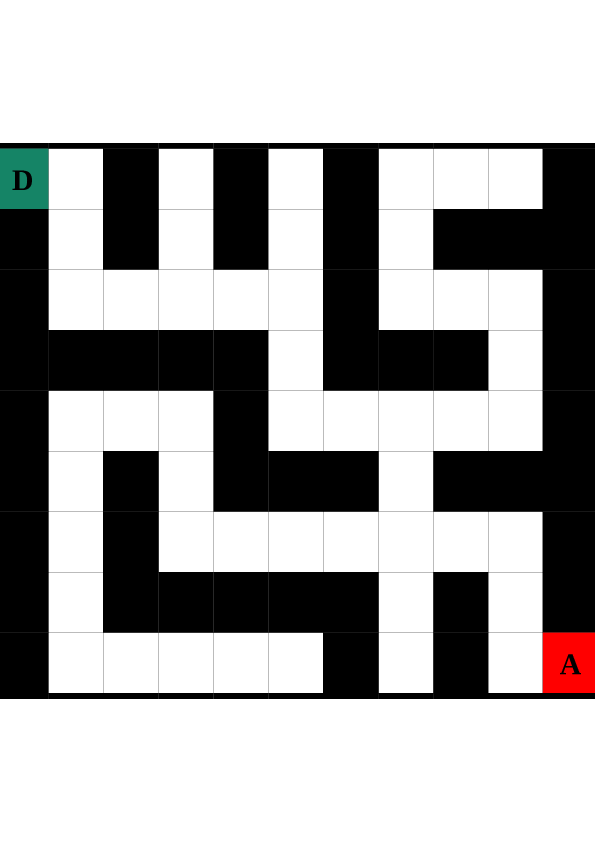
\includegraphics[width=\linewidth]{../diapos/page1.png}}    
  \end{minipage}
\end{frame} % Titre

\begin{frame}
  \frametitle{Table des matières}
  \tableofcontents
\end{frame} % toc

\section{Quel algorithme pour résoudre quel problème?}
\subsection{Choix du problème}
\begin{frame} 
  \frametitle{Un labyrinthe, plusieurs problèmes}
  \begin{itemize}
  \item<1-> Cherche-t-on un chemin quelconque?
    \begin{itemize}
    \item<2-> Oui, on ne traversera le labyrinthe qu'une seule fois.
    \item<2-> \textbf<3->{On veut le chemin le plus court}, pour peut-être le réutiliser.
    \end{itemize}
  \item<4-> Connait-on les coordonnées de la sortie dès le départ?
    \begin{itemize}
    \item<5-> \textbf<6->{Oui, et cette information pourra nous aider.}
    \item<5-> Non, le lieu de la sortie partie des inconnues.
    \end{itemize}
  \end{itemize}
\end{frame} % choix du problème

\subsection{Choix de l'Algorithme}
\begin{frame}
  \frametitle{Un problème, plusieurs solutions}
  \begin{itemize}
  \item<1-> Breadth-First Search
    \begin{itemize}
    \item garantit de trouver une solution si elle existe
    \item solution optimale si tous les pas sont égaux
    \end{itemize}
  \item<2-> Dijkstra
    \begin{itemize}
    \item choisit où explorer selon les distances déjà parcourues
    \item garantit de trouver le plus court chemin
    \end{itemize}    
  \item<3-> A*
    \begin{itemize}
    \item nécessite de connaître les coordonnées de la sortie
    \item choisit où explorer selon les distances déjà parcourues et la distance
      à la sortie
    \end{itemize}
  \end{itemize}
\end{frame}

\section{Algorithme A*}
\subsection{Heuristique}
\begin{frame}
  \frametitle{Heuristique}
  La distance restante depuis une cellule jusqu'à l'arrivée doit être estimée
  \textit{sans jamais surestimer}.
  \begin{itemize}
  \item<2->{La \textbf{distance de Manhattan} $|\Delta x| + |\Delta y|$
    est un bon estimateur sur une grille carrée.}
  \par
  \item<3>{Une \textbf{heuristique nulle} ramène A* à l'algorithme de Dijkstra
      (ou Breadth-First Search sur grille carrée).}
  \end{itemize}
\end{frame}

\subsection{Structure de données ``Priority Queue''}
\begin{frame}
  \frametitle{Priority Queue}
  \begin{itemize}
  \item Structure permettant insertion avec priorité et ``pop'' rapide de
    l'élément prioritaire (ici la priorité est à l'élément de valeur plus basse)
  \item Implémentation en Python avec le module \textit{heapq}
  \item Un élément est un tuple (heuristique, numéro, contenu), ainsi en cas
    d'heuristique égale, le numéro le plus bas (insertion plus ancienne) donne
    la priorité
  \end{itemize}
\end{frame}
\begin{frame}
  \frametitle{Priority Queue pour A*}
  \begin{itemize}
  \item<1-> La priorité d'un noeud est le \textbf{coût heuristique} pour aller de
    l'entrée à la sortie en passant par ce noeud.
  \item<2-> Un élément de la queue a comme attributs l'identité du noeud, le
    \textbf{coût réel} pour y accéder et son prédecesseur
  \item<3-> La queue est initialisée avec le noeud de départ et un coût nul.
  \end{itemize}
\end{frame}

\subsection{Pseudo-Code}
\begin{frame}
  \frametitle{Algorithme A*}
  \begin{block}{pseudo-code}
    Tant que la queue prioritaire n'est pas vide,
    \begin{itemize}
    \item<2-> extraire (pop) la cellule prioritaire de la queue
    \item<3-> si la cellule est la cellule d'arrivée, retourner le chemin qui y amène
          (via backtracking sur la liste de cellules déjà traitées)
    \item<4-> sinon,
      \begin{itemize}
      \item<4-> ajouter à la queue prioritaire chaque voisin admissible\footnote{un
          voisin est admissible s'il n'est pas dans la liste de cellules déjà
          traitées} de la cellule
      \item<5-> ajouter à la liste des cellules traitées la cellule actuelle
      \end{itemize}
    \end{itemize}    
  \end{block}
\end{frame}

\subsection{Idée de preuve}
\begin{frame}
  \frametitle{Idée de preuve}
  Si l'heuristique sous-estime le coût du chemin futur, alors on arrive à un
  noeud toujours par un chemin de distance minimale d'abord.

  [à expliquer]
\end{frame}

\subsection{Exemple de résolution}
\begin{frame}
  \frametitle{Exemple de résolution}
  \begin{minipage}{.4\textwidth}    
    \only<1>{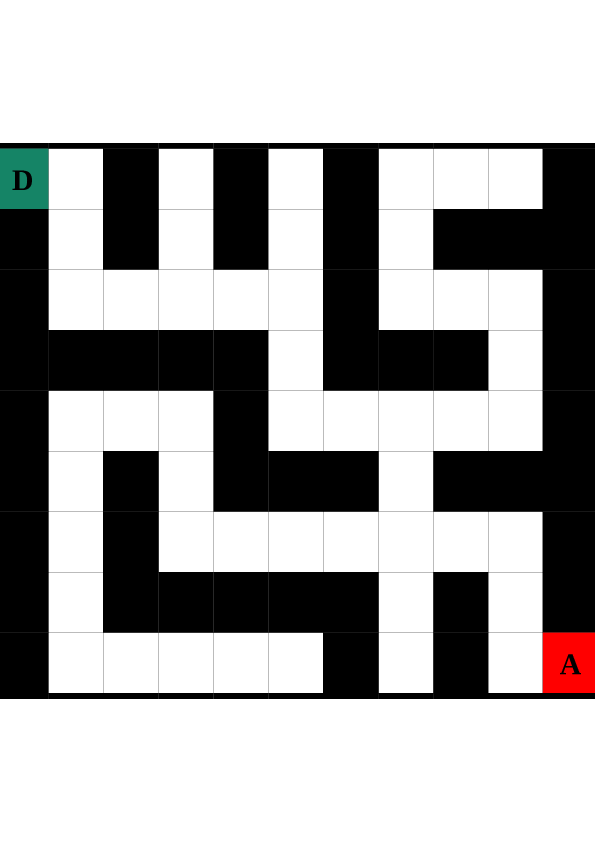
\includegraphics[width=\linewidth]{../diapos/page1.png}}
    \only<2>{\includegraphics[width=\linewidth]{../diapos/page3.png}}
    \only<3>{\includegraphics[width=\linewidth]{../diapos/page2.png}}
    \setcounter{pngnumber}{7}
    \forloop{onlynumber}{4}{\value{onlynumber} < 46}{
      % \only<\arabic{onlynumber}>{only \theonlynumber, png \thepngnumber}\par
      \only<\arabic{onlynumber}>{\includegraphics[width=\linewidth]{../diapos/page\arabic{pngnumber}.png}}
      \stepcounter{pngnumber}
    }
  \end{minipage}
  \quad
  \begin{minipage}{.55\textwidth}
    \only<1>{\textbf{Objectif}\par
      Trouver le chemin le plus court entre le \textbf{D}épart
      et l'\textbf{A}rrivée}
    \only<2>{Chaque noeud est à une distance réelle de l'arrivée, mais ces
      distances ne sont pas encore connues.}
    \only<3>{Le départ est mis en file d'attente, avec une priorité 0.}
    \only<4>{Le seul voisin est évalué:
      \begin{itemize}
      \item coût réel pour y accéder: \textcolor{green}1
      \item coût heuristique pour la suite: \textcolor{red}{17}
      \item coût heuristique total (priorité): 18
      \end{itemize}
    }
    \only<5-26>{
      Légende:
      \begin{itemize}
      \item\textcolor{green}{coût réel jusqu'ici}
      \item\textcolor{red}{coût heuristique pour la suite}
      \item {coût heuristique total}
      \end{itemize}
      \medskip
      L'algorithme poursuit son chemin.}
    \onslide<15,19,20>{\par Parfois deux choix ont la même priorité.}
    \only<27->{Un chemin vers la sortie a été trouvé!}
    \onslide<28->{Backtracking pour reconstituer le chemin}
  \end{minipage}
\end{frame}

\section{Complexité}
\begin{frame}
  \frametitle{Complexité}
  Le pire des cas sera réalisé par un labyrinthe dont le meilleur chemin revient
  souvent en arrière (s'éloigne de l'arrivée). Dans ce cas, aucun gain n'est
  réalisé par rapport à l'algorithme de Dijsktra.
\end{frame}

\section{Tests avec Python}
\begin{frame}
  \frametitle{Tests avec Python}
\end{frame}

\section{Conclusion}
\begin{frame}
  \frametitle{Conclusion}
  \begin{itemize}
  \item \ldots
  \item Robot-Aspirateur
  \end{itemize}
\end{frame}

\section*{-- fin des vrais slides --}

%\section{-- fin des vrais slides --}
\begin{frame}
  \begin{center}
    {\Huge Fin des vrais slides}
    \par\bigskip
    Tout ce qui suit sont des essais de mise en page, etc.
  \end{center}
\end{frame}

%\subsection{Test de pseudo-code}
\begin{frame}
  \frametitle{Effets simples dans beamer}
  \begin{block}{ceci est un bloc}
    On peut pseudo-inclure du code.
  \end{block}
  \begin{definition}
    Le pseudo-code est un outil de communication entre humains.
  \end{definition}
  \begin{example}
    Ce qui suit est en fait du vrai code: un outil de communication humain-machine.
  \end{example}
  \begin{semiverbatim}
    print("Hello, world!")
  \end{semiverbatim}
  \begin{alertblock}{Attention!}
    Ce slide ne doit pas être gardé dans la vraie présentation!
  \end{alertblock}
\end{frame}

%\subsection{Essai importation depuis l'odt}
\begin{frame}
  \frametitle{Tentons d'importer}
  \begin{minipage}{.4\textwidth}    
    \only<1>{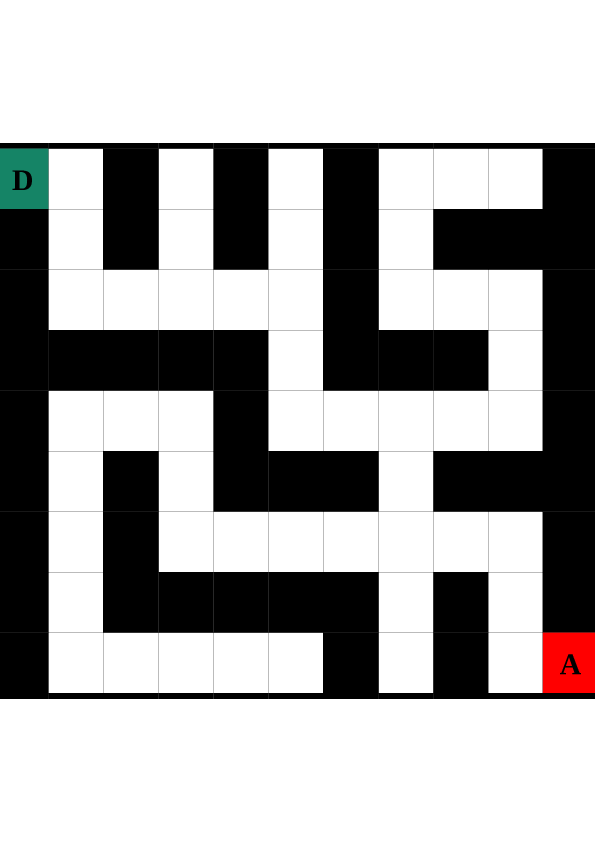
\includegraphics[width=\linewidth]{../diapos/page1.png}}
    \only<2>{\includegraphics[width=\linewidth]{../diapos/page2.png}}
    \only<3>{\includegraphics[width=\linewidth]{../diapos/page3.png}}
  \end{minipage}
  \quad
  \begin{minipage}{.4\textwidth}
    \only<1>{Ceci est un labyrinthe.}
    \onslide<2-3>{Il a un coût réel ``c''.}
    \par\medskip
    \onslide<3>{Voici le nombre de pas nécessaires à atteindre chaque case.}
  \end{minipage}
\end{frame}

%\subsection{Exemple}
\begin{frame}
\frametitle{Labyrinthe de démonstration}

\begin{tikzpicture}[scale=.5]
  % Grid
  \draw[lightgray!20] (0,0) grid (8,8);
  
  % Puzzle
  \draw[line width=3pt,
  cap=round,
  rounded corners=1pt,
  draw=black!75] (-0.5,-0.5) -| (8.5,8.5)
  (7.5,8.5)-|(-0.5,0.5) -- (0.5,0.5) (-0.5,2.5)-|(0.5,4.5)
  (0.5,5.5)|-(4.5,7.5)|-(3.5,3.5)|-(2.5,2.5)|-(3.5,1.5)
  (8.5,0.5)--(6.5,0.5)
  (5.5,0.5)-|(3.5,-0.5)
  (3.5,0.5)-|(1.5,3.5)-|(2.5,5.5)
  (2.5,4.5)-|(3.5,6.5)-|(1.5,4.5)
  (7.5,8.5)|-(5.5,6.5)--(5.5,7.5)
  (6.5,7.5)--(6.5,8.5)
  (8.5,3.5)-|(6.5,4.5)-|(7.5,5.5)
  (6.5,5.5)-|(5.5,2.5)--(4.5,2.5)
  (5.5,2.5)-|(7.5,1.5)--(4.5,1.5)
  (5.5,4.5)--(4.5,4.5)
  (1.5,1.5)--(0.5,1.5)
  (1.5,7.5)--(1.5,8.5);
  
  % Start and End Points
  \onslide<2>{\draw[-latex,line width=3pt,red] (-1,0)--(0,0);}
  \onslide<3>{\draw[-latex,line width=3pt,red] (8,8) -- (8,9);}
\end{tikzpicture}
\end{frame}
\end{document}